\section{Earlier Background Studies}
\label{app:bkg_CR_phys14}

We present the yields and \met distributions in the control regions defined in Sec.~\ref{subsec:bkg_hadronic} for studies done for the center-of-mass energy of $s=\sqrt{8\:\TeV\:}$. The main backgrounds in the hadronic channel are, as in the $13\:\TeV\:$ analysis, semileptonic $\ttbar$, $\Wjets$, and $\Z(\Nu\Nu)+$jets.

\subsubsection{Control region for \texorpdfstring{$\ttbar$}{ttbar}}
\label{subsubsec:bkg_hadronic_ttbar_8tev}

\begin{table}[!ht]
\centering
\begin{tabular}{|c|r|r|r|r|}
\hline
  Process & \multicolumn{1}{|c|}{Inclusive} &\iffalse \multicolumn{1}{|c|}{Bst,Bst} & \multicolumn{1}{|c|}{Bst,Res} & \fi \multicolumn{1}{|c|}{Res,Res} \\
\hline
  \Z\To\Lep\Lep          & $   3.41 \pm  0.29$ & \iffalse$ 0.17 \pm 0.03$ & $  2.41 \pm  0.33$ & \fi$  2.86 \pm  0.27$ \\
  Single \Top            & $ 183.25 \pm  5.68$ & \iffalse$ 6.96 \pm 1.12$ & $ 94.99 \pm  4.13$ &\fi $140.05 \pm  4.96$ \\
  \Wjets                 & $ 130.53 \pm  4.69$ & \iffalse$ 7.04 \pm 0.48$ & $106.84 \pm  3.60$ &\fi $109.44 \pm  4.51$ \\
  $\ttbar+V$             & $   9.75 \pm  0.37$ & \iffalse$ 1.80 \pm 0.16$ & $  8.61 \pm  0.35$ & \fi$  5.33 \pm  0.28$ \\
  $\ttbar(\mbox{had})$   & $   0.33 \pm  0.23$ & \iffalse$ 0.16 \pm 0.16$ & $  0.49 \pm  0.28$ & \fi$  0.00 \pm  0.00$ \\
  $\ttbar(1\Lep)$        & $ 848.86 \pm 11.78$ & \iffalse$37.26 \pm 2.47$ & $618.91 \pm 10.06$ & \fi$598.48 \pm  9.89$ \\
  $\ttbar(2\Lep)$        & $  82.53 \pm  3.67$ & \iffalse$ 3.11 \pm 0.71$ & $ 30.72 \pm  2.24$ & \fi$ 68.48 \pm  3.35$ \\
\hline
  SM expected            & $1258.65 \pm 14.38$ & \iffalse$56.52 \pm 2.85$ & $862.97 \pm 11.68$ & \fi$924.64 \pm 12.41$ \\
\hline
  $M_\chi=1\:\GeV$       & $  14.27 \pm  0.77$ & \iffalse$ 0.62 \pm 0.16$ & $  7.53 \pm  0.56$ &\fi $ 10.24 \pm  0.65$ \\
\hline
\end{tabular}
\caption{Expected yields for $5\:\ifb$ in the $\ttbar$ control region for the hadronic channel.}
\label{tab:hadronic_bkg_tt1l_yields_8tev}
\end{table}

\begin{figure}[htbp]
  \centering
  \includegraphics[width=0.48\textwidth]{figures/hadronic-incl-tt1l-fmet.pdf}
  \includegraphics[width=0.48\textwidth]{figures/hadronic-incl-tt1l-fmetlog.pdf}
    \caption{The $\met$ distribution in the $\ttbar$ control region for the hadronic channel.}
  \label{fig:incl_hadronic_1l_fmet}
\end{figure}


\begin{table}[!ht]
\centering
\begin{tabular}{|c|r|r|r|r|}
\hline
  Process & \multicolumn{1}{|c|}{Inclusive} &\iffalse \multicolumn{1}{|c|}{Bst,Bst} & \multicolumn{1}{|c|}{Bst,Res} & \fi \multicolumn{1}{|c|}{Res,Res} \\
\hline
  \Z\To\Lep\Lep          & $  12.20 \pm  0.57$ & \iffalse$ 0.19 \pm 0.03$ & $  1.37 \pm 0.16$ & \fi $  10.73 \pm  0.54$ \\
  \Z\To\Nu\Nu            & $1993.44 \pm  9.18$ &\iffalse $28.91 \pm 0.51$ & $222.44 \pm 2.47$ & \fi $1753.95 \pm  8.84$ \\
  Single \Top            & $  20.30 \pm  1.70$ &\iffalse $ 0.83 \pm 0.37$ & $  2.92 \pm 0.68$ & \fi $  16.96 \pm  1.54$ \\
  \Wjets                 & $1254.64 \pm 16.68$ &\iffalse $20.64 \pm 1.03$ & $143.99 \pm 4.73$ & \fi $1099.65 \pm 15.97$ \\
  QCD                    & $   0.00 \pm  0.00$ &\iffalse $ 0.00 \pm 0.00$ & $  0.00 \pm 0.00$ & \fi $   0.00 \pm  0.00$ \\
  $\ttbar+V$             & $   4.53 \pm  0.25$ & \iffalse$ 0.52 \pm 0.09$ & $  1.78 \pm 0.16$ & \fi $   2.44 \pm  0.19$ \\
  $\ttbar(\mbox{had})$   & $   0.00 \pm  0.00$ &\iffalse $ 0.00 \pm 0.00$ & $  0.00 \pm 0.00$ & \fi $   0.00 \pm  0.00$ \\
  $\ttbar(1\Lep)$        & $ 141.20 \pm  4.80$ & \iffalse$ 4.90 \pm 0.90$ & $ 35.79 \pm 2.42$ & \fi $ 103.45 \pm  4.11$ \\
  $\ttbar(2\Lep)$        & $  12.91 \pm  1.45$ & \iffalse$ 0.16 \pm 0.16$ & $  2.78 \pm 0.67$ & \fi $  10.13 \pm  1.29$ \\
\hline
  SM expected            & $3439.22 \pm 19.78$ & \iffalse$56.16 \pm 1.51$ & $411.06 \pm 5.94$ & \fi $2997.31 \pm 18.83$ \\
\hline
  $M_\chi=1\:\GeV$       & $ 121.79 \pm  2.24$ & \iffalse$11.72 \pm 0.69$ & $ 45.78 \pm 1.37$ & \fi $  67.46 \pm  1.67$ \\
\hline
\end{tabular}
\caption{Expected yields for $5\:\ifb$ in the $V+$jets control region for the hadronic channel.}
\label{tab:hadronic_bkg_vjets_yields}
\end{table}

\begin{figure}[htbp]
  \centering
  \includegraphics[width=0.48\textwidth]{figures/hadronic-incl-0b-fmet.png}
  \includegraphics[width=0.48\textwidth]{figures/hadronic-incl-0b-fmetlog.png}
  \caption{The $\met$ distribution in the $V+$jets control region for the hadronic channel.}
  \label{fig:incl_hadronic_0b_met}
\end{figure}



\begin{table}[!ht]
\centering
\begin{tabular}{|c|r|r|r|r|}
\hline
  Process &  \multicolumn{1}{|c|}{Inclusive} &\iffalse \multicolumn{1}{|c|}{Bst,Bst} & \multicolumn{1}{|c|}{Bst,Res} & \fi \multicolumn{1}{|c|}{Res,Res} \\
\hline
  \Z\To\Lep\Lep          & $ 101.58 \pm  1.73$ & \iffalse$ 1.15 \pm 0.09$ & $ 10.40 \pm  0.42$ & \fi $  90.58 \pm  1.68$ \\
  Single \Top            & $ 171.78 \pm  5.38$ & \iffalse$ 2.60 \pm 0.68$ & $ 27.49 \pm  2.18$ & \fi$ 142.47 \pm  4.89$ \\
  \Wjets                 & $4778.24 \pm 33.41$ &\iffalse $53.69 \pm 1.54$ & $504.80 \pm  8.51$ &\fi $4238.41 \pm 32.28$ \\
  $\ttbar+V$             & $   6.71 \pm  0.31$ & \iffalse$ 0.55 \pm 0.09$ & $  2.39 \pm  0.19$ &\fi $   3.94 \pm  0.24$ \\
  $\ttbar(\mbox{had})$   & $   0.33 \pm  0.23$ &\iffalse $ 0.16 \pm 0.16$ & $  0.16 \pm  0.16$ & \fi$   0.00 \pm  0.00$ \\
  $\ttbar(1\Lep)$        & $1003.13 \pm 12.80$ &\iffalse $20.59 \pm 1.83$ & $217.36 \pm  5.96$ & \fi$ 772.86 \pm 11.24$ \\
  $\ttbar(2\Lep)$        & $  81.55 \pm  3.65$ & \iffalse$ 0.82 \pm 0.37$ & $ 13.40 \pm  1.48$ &\fi $  67.66 \pm  3.33$ \\
\hline
  SM expected            & $6143.32 \pm 36.41$ &\iffalse $79.57 \pm 2.52$ & $776.02 \pm 10.73$ & \fi$5315.92 \pm 34.73$ \\
\hline
  $M_\chi=1\:\GeV$       & $   5.76 \pm  0.49$ &\iffalse $ 0.29 \pm 0.11$ & $  1.60 \pm  0.26$ & \fi$   3.95 \pm  0.40$ \\
\hline
\end{tabular}
\caption{Expected yields for $5\:\ifb$ in the $\Wjets$ control region for the hadronic channel.}
\label{tab:hadronic_bkg_wjets_yields}
\end{table}

\begin{figure}[htbp]
  \centering
  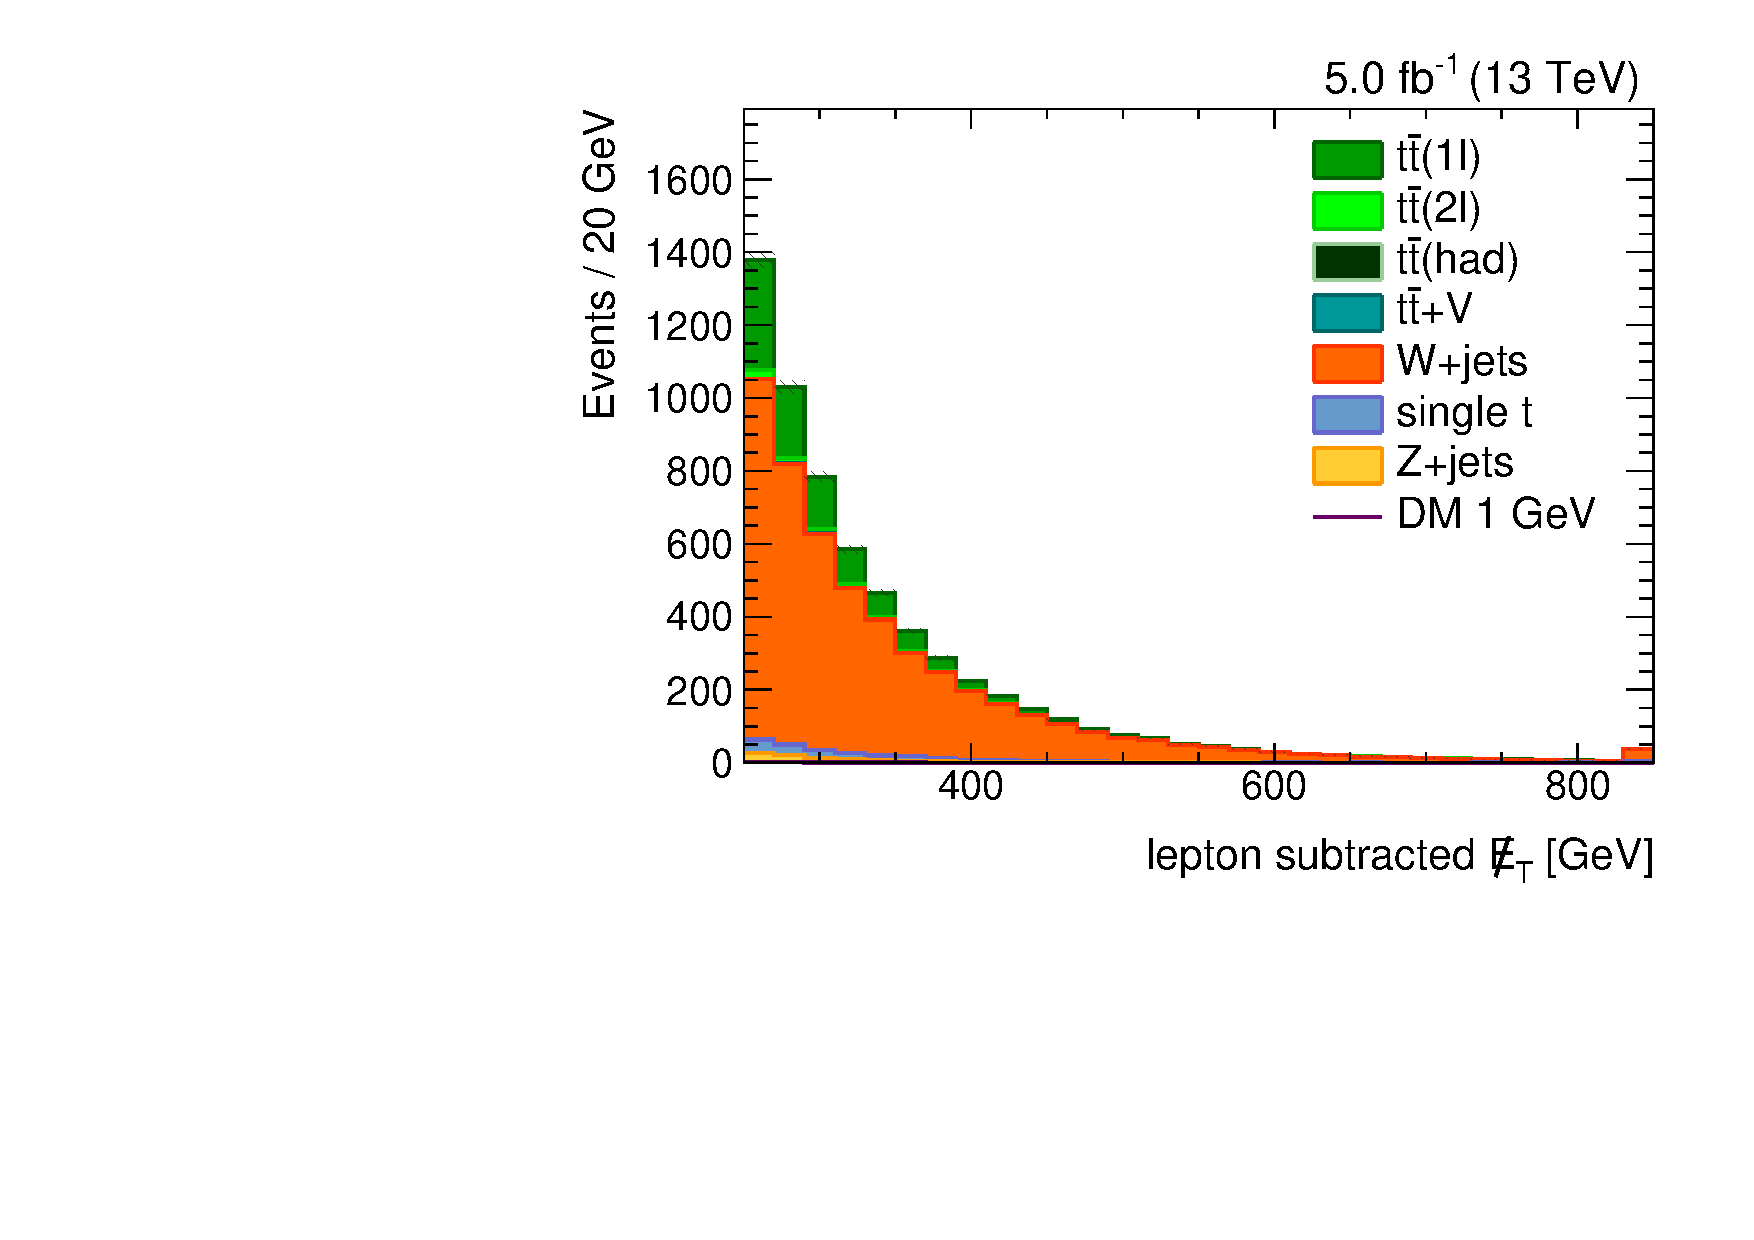
\includegraphics[width=0.48\textwidth]{figures/hadronic-incl-1l0b-fmet.pdf}
  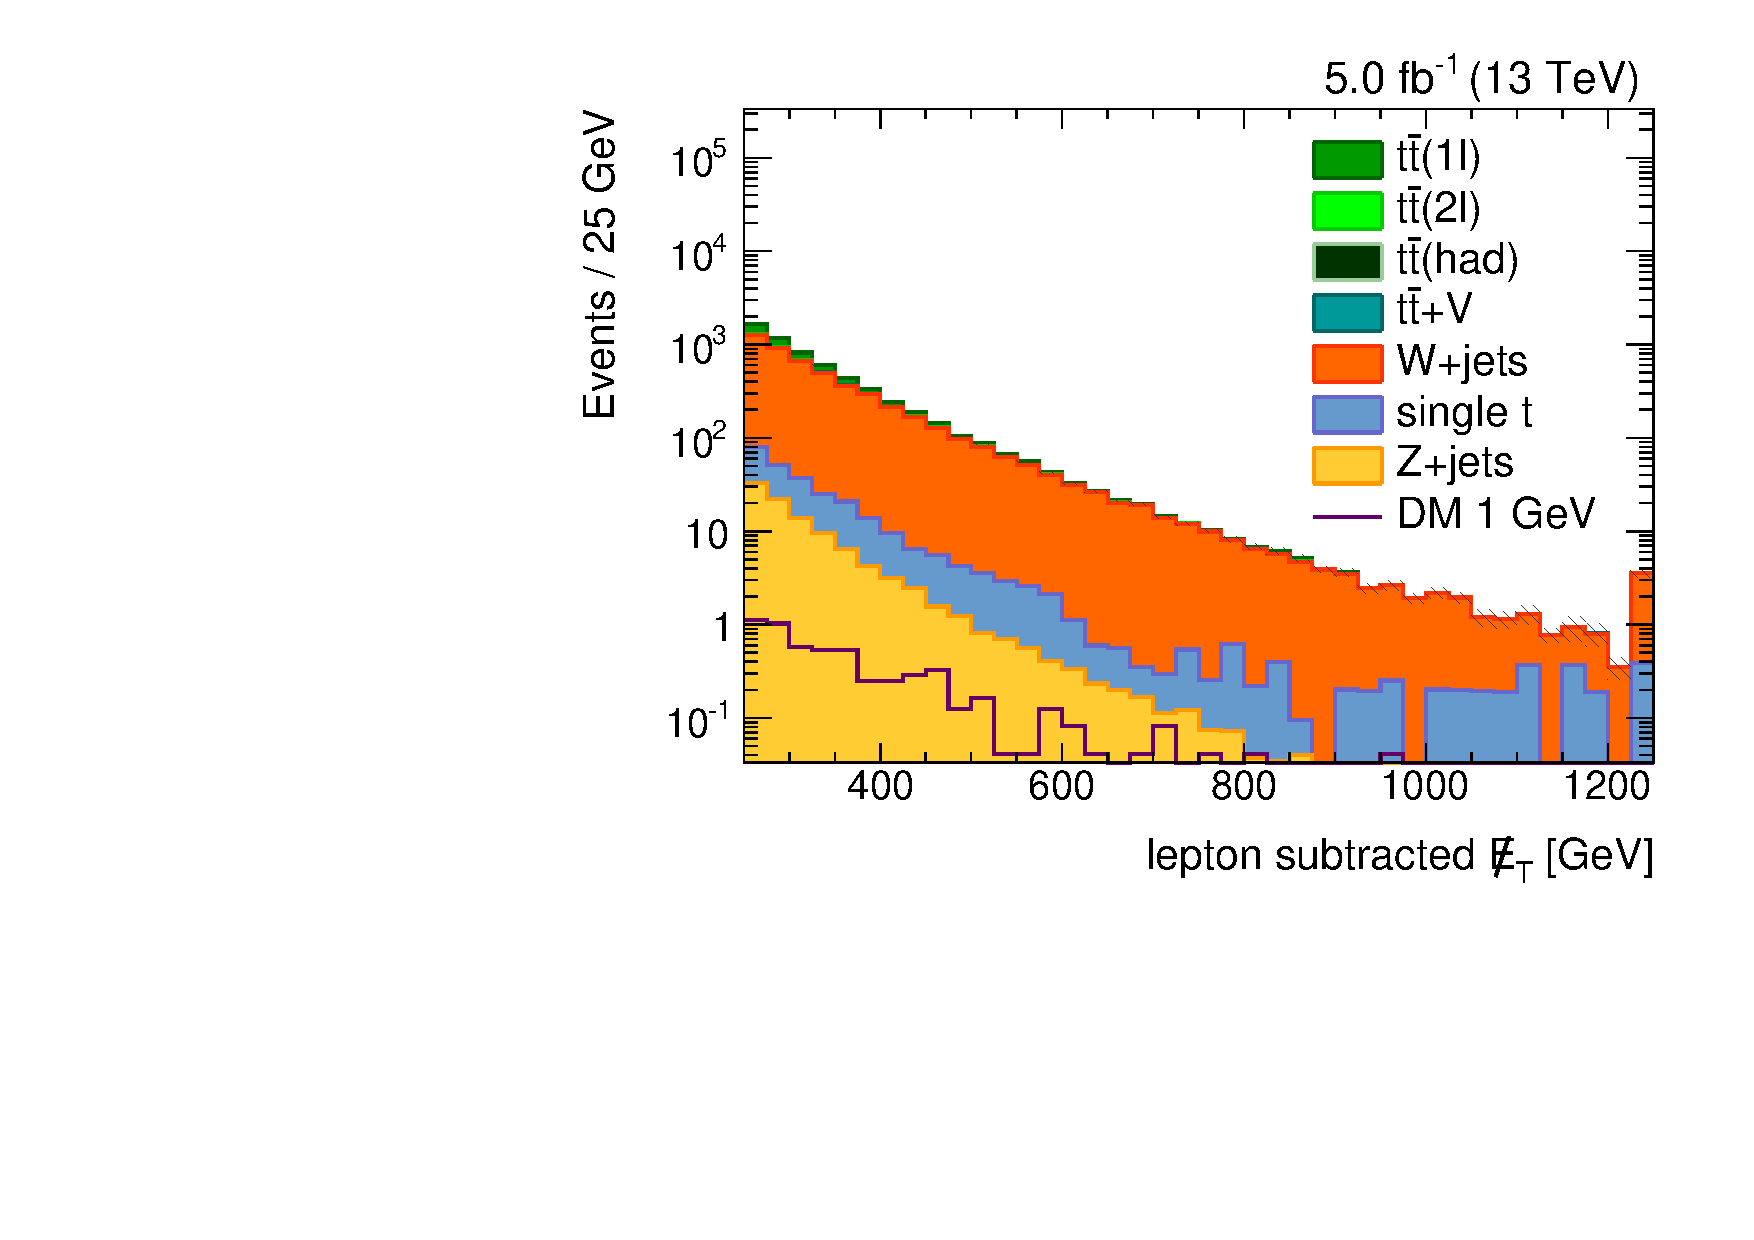
\includegraphics[width=0.48\textwidth]{figures/hadronic-incl-1l0b-fmetlog.pdf}
  \caption{The $\met$ distribution in the $\Wjets$ control region for the hadronic channel.}
  \label{fig:incl_hadronic_1l0b_fmet}
\end{figure}



\begin{table}[!ht]
\centering
\begin{tabular}{|c|r|r|r|r|}
\hline
  Process & \multicolumn{1}{|c|}{Inclusive} &\iffalse \multicolumn{1}{|c|}{Bst,Bst} & \multicolumn{1}{|c|}{Bst,Res} & \fi \multicolumn{1}{|c|}{Res,Res} \\
\hline
  \Z\To\Lep\Lep          & $420.00 \pm 3.11$ &\iffalse $4.00 \pm 0.13$ & $44.12 \pm 0.82$ &\fi $373.31 \pm 3.00$ \\
  Single \Top            & $  0.91 \pm 0.41$ &\iffalse $0.00 \pm 0.00$ & $ 0.00 \pm 0.00$ & \fi $  0.91 \pm 0.41$ \\
  \Wjets                 & $  0.17 \pm 0.11$ &\iffalse $0.00 \pm 0.00$ & $ 0.00 \pm 0.00$ & \fi $  0.17 \pm 0.11$ \\
  $\ttbar+V$             & $  1.03 \pm 0.12$ &\iffalse $0.00 \pm 0.00$ & $ 0.41 \pm 0.08$ & \fi $  9.48 \pm 1.24$ \\
  $\ttbar$               & $ 10.95 \pm 1.34$ & \iffalse$0.11 \pm 0.04$ & $ 1.47 \pm 0.49$ & \fi $  0.55 \pm 0.09$ \\
\hline
  SM expected            & $433.06 \pm 3.41$ &\iffalse $4.12 \pm 0.13$ & $46.00 \pm 0.96$ &\fi  $384.43 \pm 3.27$ \\
\hline
  $M_\chi=1\:\GeV$       & $  0.04 \pm 0.04$ &\iffalse $0.00 \pm 0.00$ & $ 0.00 \pm 0.00$ &\fi  $  0.04 \pm 0.04$ \\
\hline
\end{tabular}
\caption{Expected yields for $5\:\ifb$ in the $\Zjets$ control region with dileptons for the hadronic channel.}
\label{tab:hadronic_bkg_zjets_yields}
\end{table}

\begin{figure}[htbp]
  \centering
  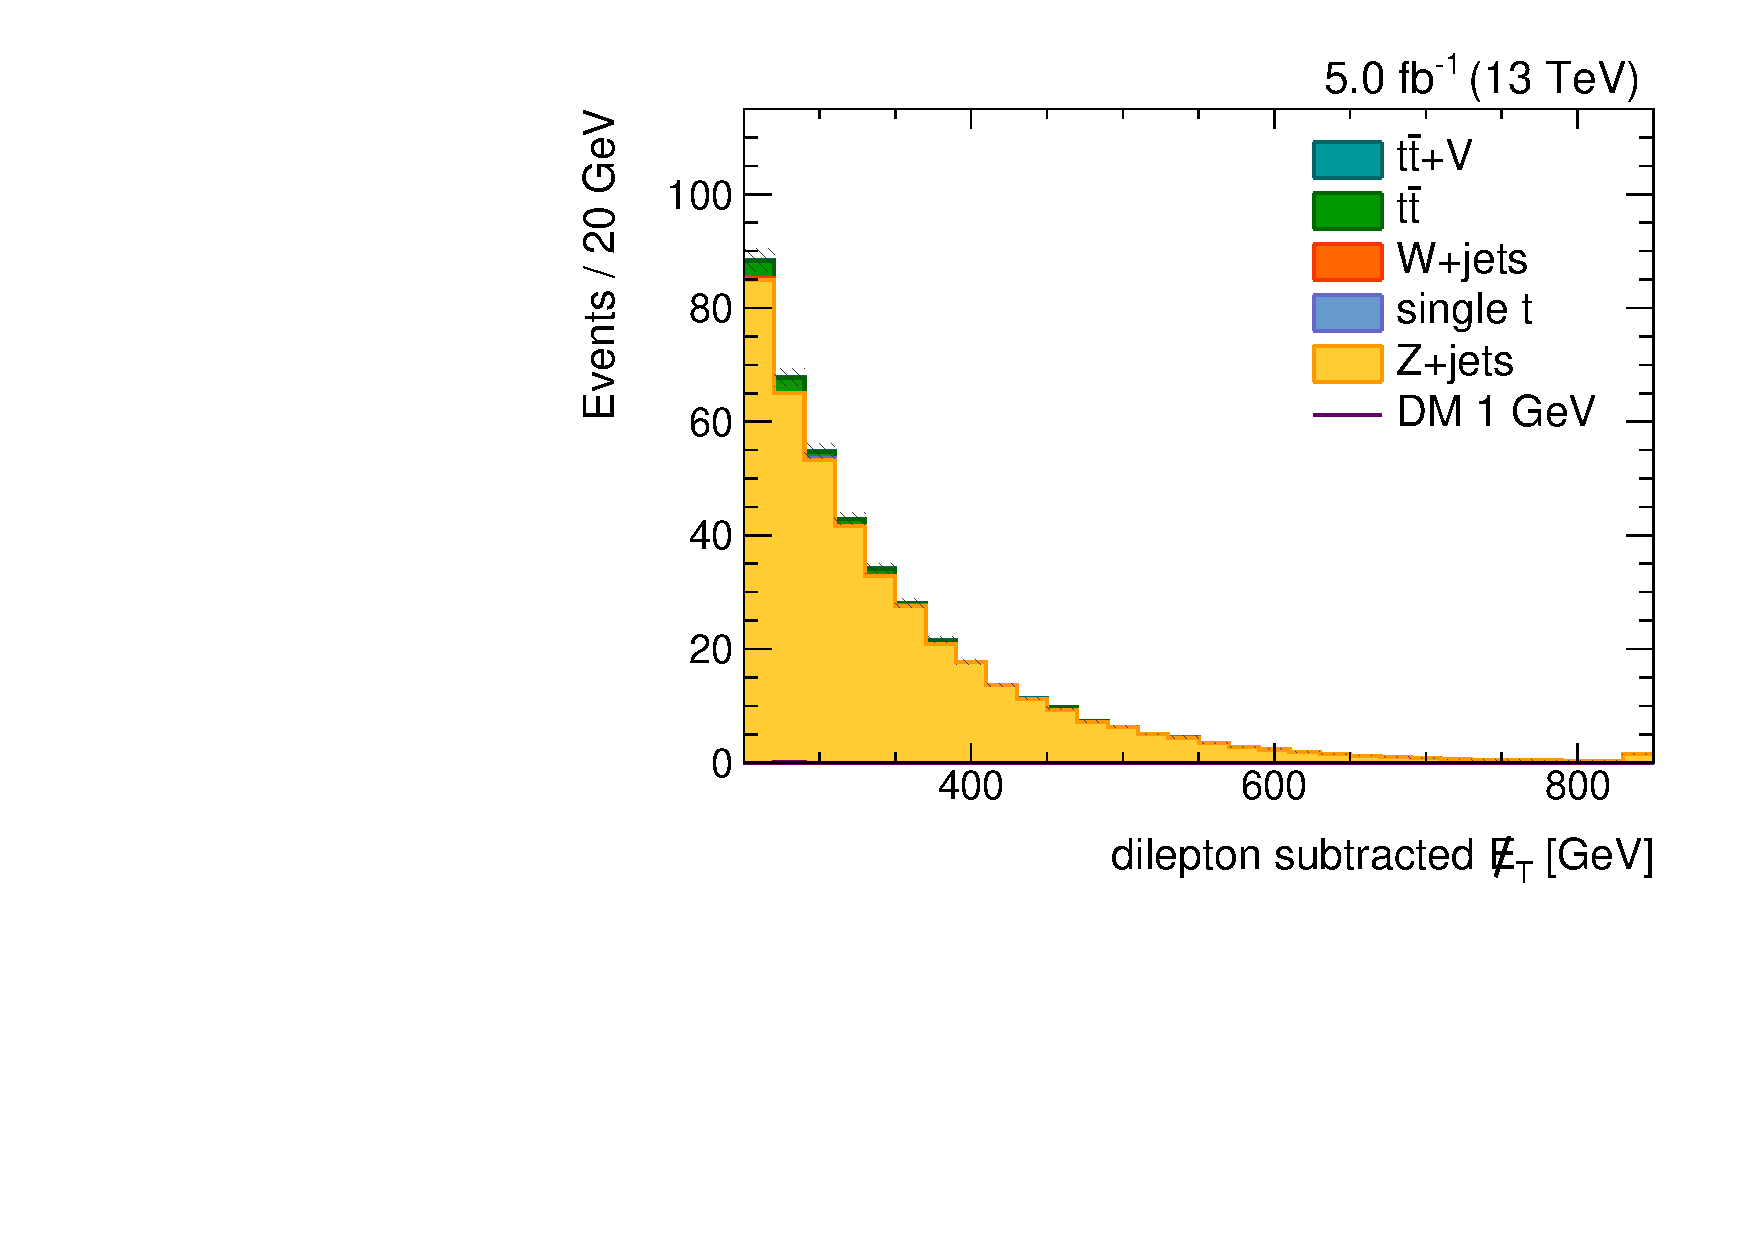
\includegraphics[width=0.48\textwidth]{figures/hadronic-incl-2l0b-fmet.pdf}
  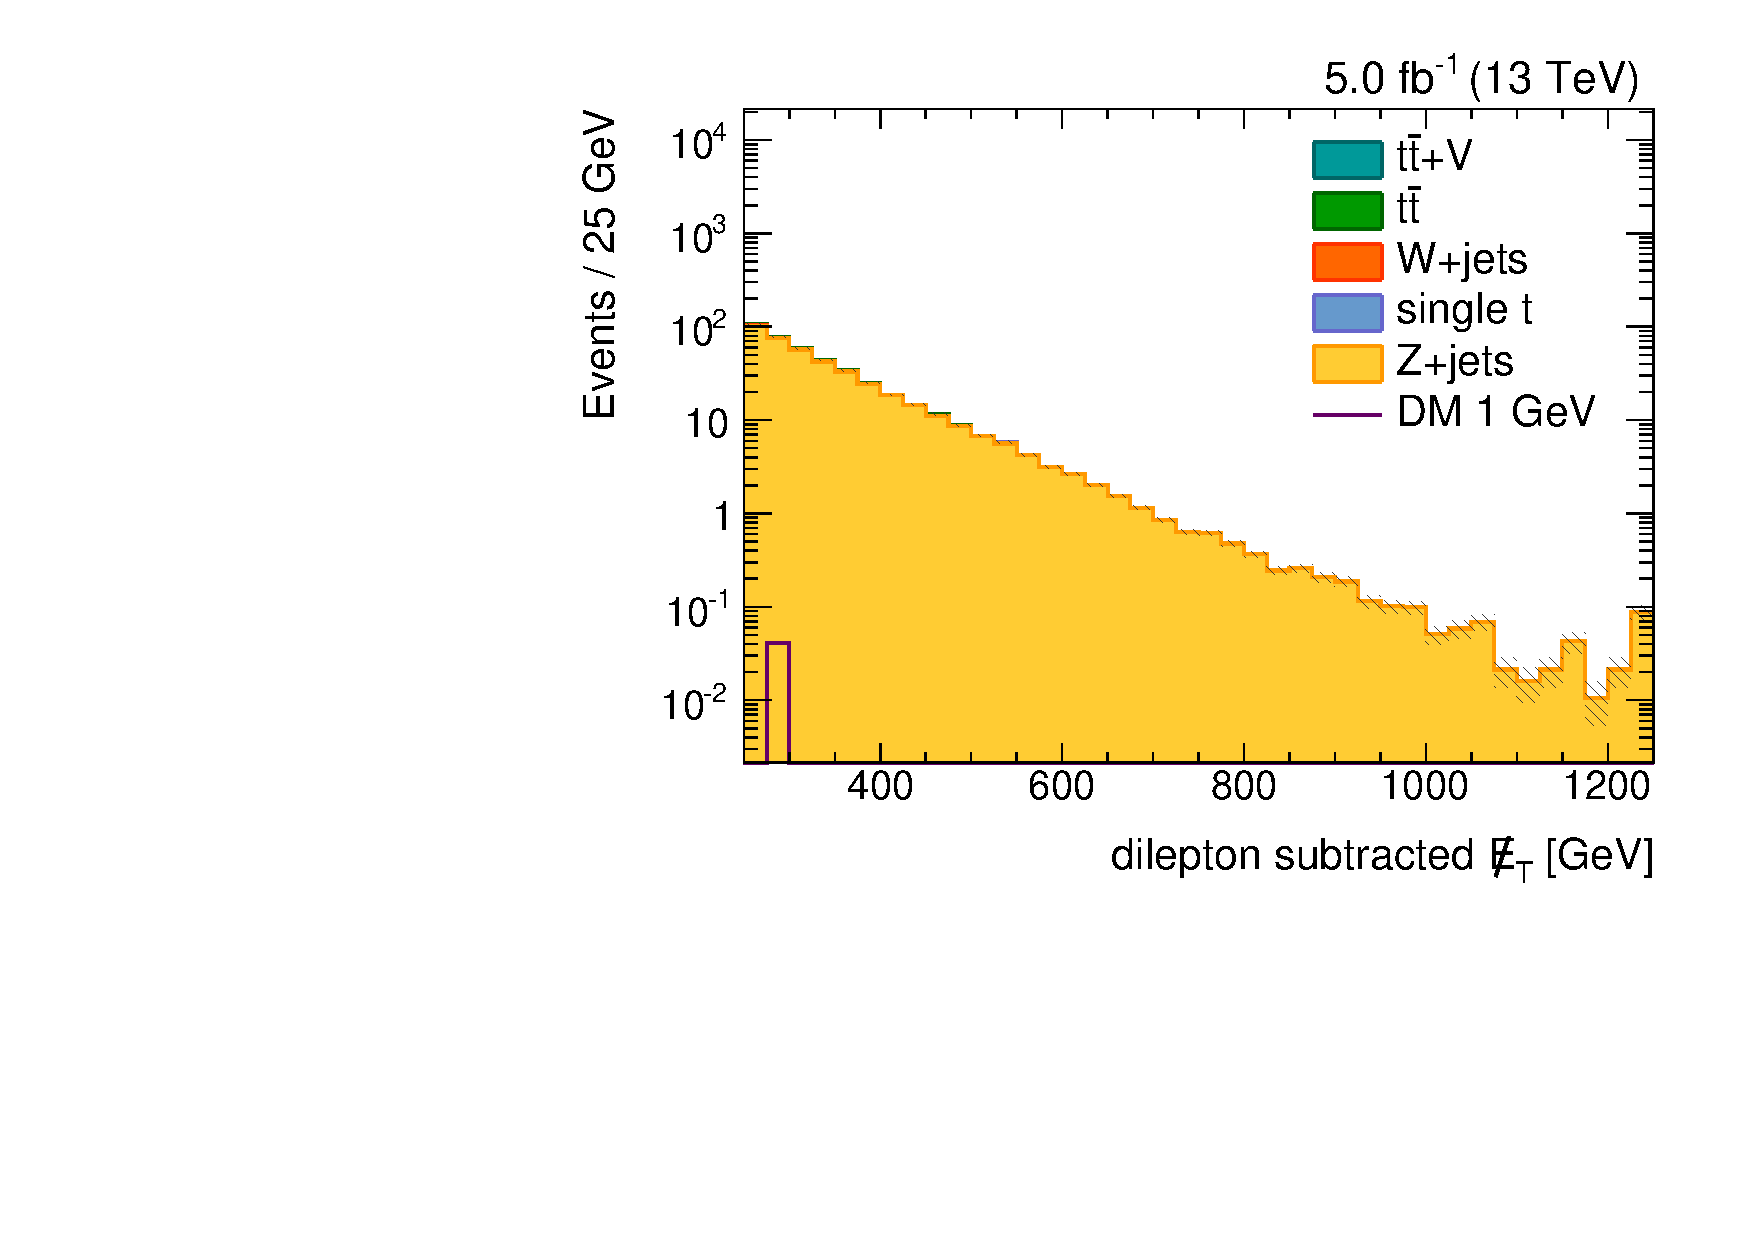
\includegraphics[width=0.48\textwidth]{figures/hadronic-incl-2l0b-fmetlog.pdf}
  \caption{The $\met$ distribution in the $\Zjets$ control region with dileptons for the hadronic channel.}
  \label{fig:incl_hadronic_2l0b_fmet}
\end{figure}



\begin{table}[!ht]
\centering
\begin{tabular}{|c|r|r|r|r|}
\hline
  Process &  \multicolumn{1}{|c|}{Inclusive} &\iffalse \multicolumn{1}{|c|}{Bst,Bst} & \multicolumn{1}{|c|}{Bst,Res} & \fi \multicolumn{1}{|c|}{Res,Res} \\
\hline
  $\gamma+$jets          & $96.53 \pm 3.94$ &\iffalse $22.73 \pm 1.97$ & $69.62 \pm 2.50$ & \fi $78.97 \pm 3.66$ \\
  QCD                    & $ 0.00 \pm 0.00$ & \iffalse$ 0.00 \pm 0.00$ & $ 2.72 \pm 2.72$ & \fi $ 0.00 \pm 0.00$ \\
\hline
  SM expected            & $96.53 \pm 3.94$ & \iffalse$22.73 \pm 1.97$ & $72.34 \pm 3.69$ & \fi $78.97 \pm 3.66$ \\
\hline
\end{tabular}
\caption{Expected yields for $5\:\ifb$ in the $\Zjets$ control region with photons for the hadronic channel.}
\label{tab:hadronic_bkg_pho_yields}
\end{table}



\begin{figure}[htbp]
  \centering
  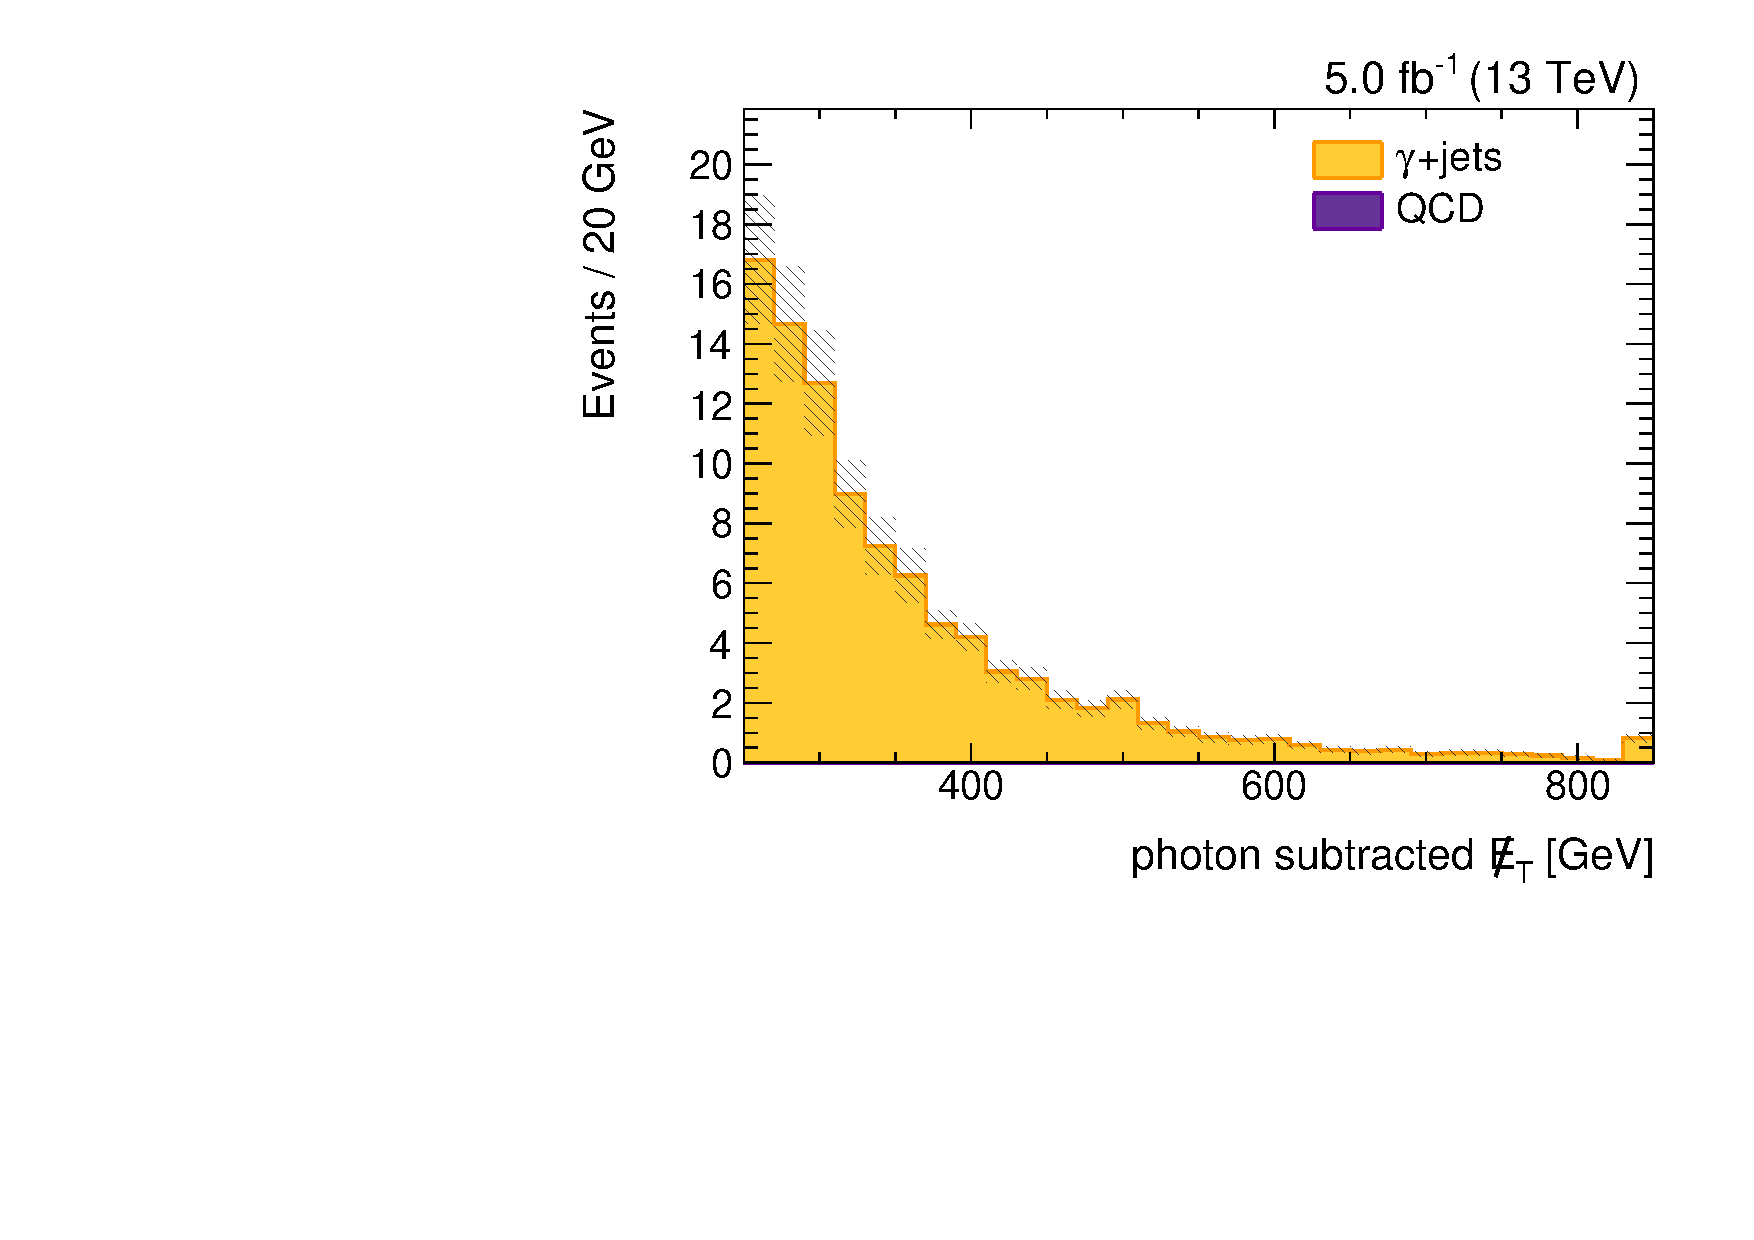
\includegraphics[width=0.48\textwidth]{figures/hadronic-incl-photon-fmet.pdf}
  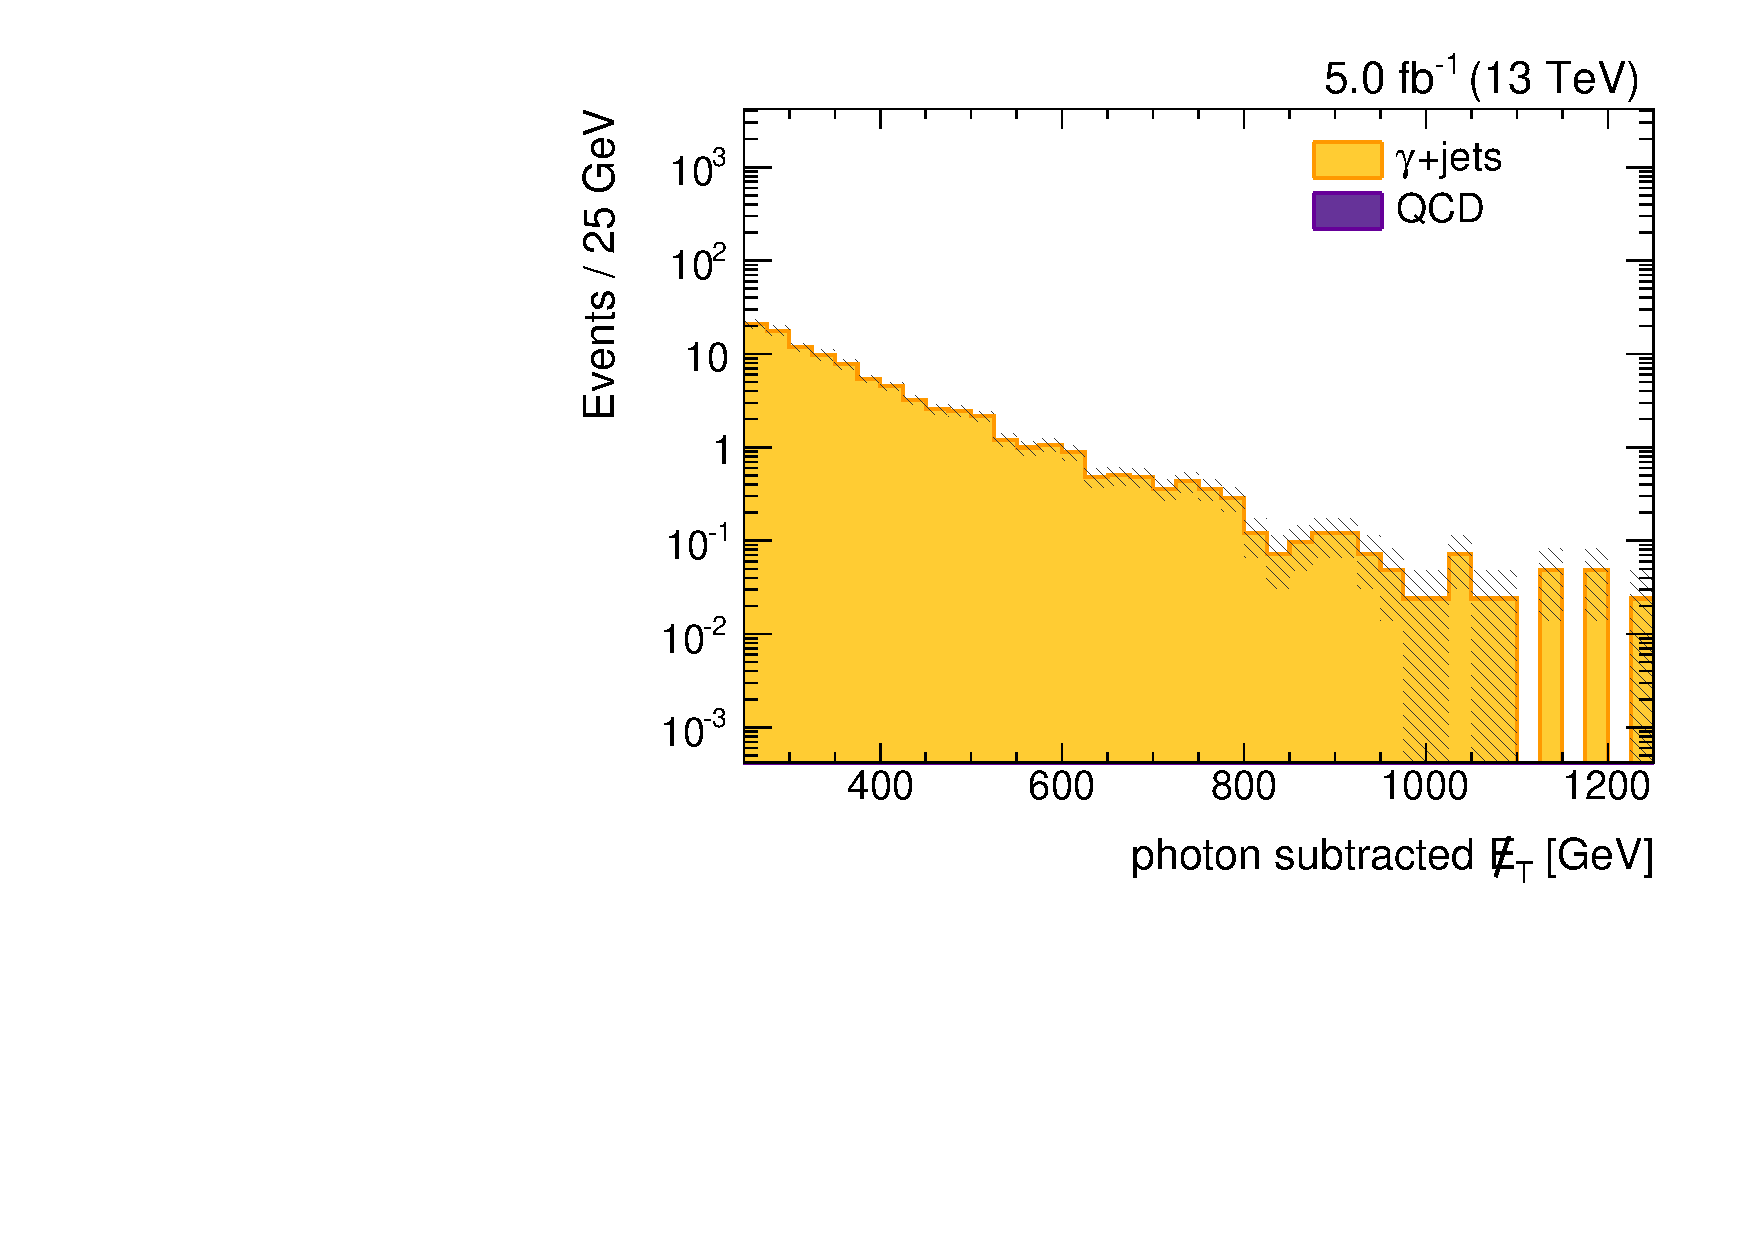
\includegraphics[width=0.48\textwidth]{figures/hadronic-incl-photon-fmetlog.pdf}
  \caption{The $\met$ distribution in the $\Zjets$ control region with photons for the hadronic channel.}
  \label{fig:incl_hadronic_pho_fmet}
\end{figure}


